		\tikzsetfigurename{Fig_module_2_1_13_Arcsine_Arccosine}

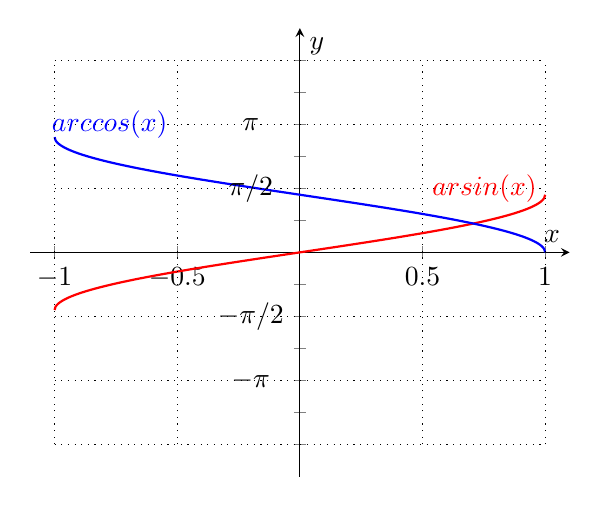
\begin{tikzpicture}
\begin{axis}[ylabel=$y$,xlabel=$x$,
axis lines=middle,
xmin=-1.1,xmax = 1.1,ymin=-350,ymax=350,
%minor x tick num = 0.5,
xtick={-1,-0.5,0,0.5,1},
domain=-1:1,
xticklabel={},
ytick={-300,-250,-200,-150,-100,-50,0,50,100,150,200,250,300}, 
yticklabel={\textcolor{white}\ticknum}
]
\addplot[samples=500,color=red,thick] {asin(x)};
\addplot[samples=500,color=blue,thick] {acos(x)};

%\addplot[samples=500,color=red,thick] {asin(-x)+200};
%\addplot[samples=500,color=red,thick] {asin(-x)-200};
\draw[dotted] (-1,100)--(1,100);
\draw[dotted] (-1,200)--(1,200);
\draw[dotted] (-1,300)--(1,300);

\draw[dotted] (-1,-100)--(1,-100);
\draw[dotted] (-1,-200)--(1,-200);
\draw[dotted] (-1,-300)--(1,-300);


\draw[](-0.2,-100) node[]{$-\pi/2$}; 
\draw[](-0.2,-200) node[]{$-\pi$}; 

\draw[](-0.2,100) node[]{$\pi/2$}; 

\draw[](0.5,100) node[right,red]{$\text{arsin}(x) $}; 


\draw[](-0.2,200) node[]{$\pi$}; 

\draw[](-0.5,200) node[left,blue]{$\text{arccos}(x) $}; 


\draw[dotted] (0.5,-300)--(0.5,300);
\draw[dotted] (-0.5,-300)--(-0.5,300);

\draw[dotted] (1,-300)--(1,300);
\draw[dotted] (-1,-300)--(-1,300);

\end{axis}
\end{tikzpicture}